% !Mode:: "TeX:UTF-8"

\documentclass{beamer}
\usepackage{ctex}
\usepackage{amsmath}
\usepackage{amssymb}
\usepackage{mathrsfs}
\usepackage{bm}
\usepackage{physics}
\usepackage{booktabs}
\usepackage{ulem}
\usepackage{graphicx} % Required for inserting images
\usepackage{tikz}
\usepackage{listings}
\usepackage{algorithm}
\usepackage{algpseudocode}
\usepackage{hyperref}

\usetikzlibrary{arrows.meta}
\usetikzlibrary{fit,positioning}
\usetikzlibrary{shadows}
\usetikzlibrary{shapes}
\usetikzlibrary{backgrounds}

\usetheme{Berkeley}
% \useoutertheme{infolines}


%% 自定义命令
\makeatletter
\providecommand{\bigsqcap}{%
  \mathop{%
    \mathpalette\@updown\bigsqcup
  }%
}
\newcommand*{\@updown}[2]{%
  \rotatebox[origin=c]{180}{$\m@th#1#2$}%
}
\makeatother

\newcommand{\IN}{\operatorname{IN}}
\newcommand{\OUT}{\operatorname{OUT}}
\newcommand{\pred}{\text{前趋于}}
\newcommand{\pot}{\preccurlyeq}

\algnewcommand\algorithmicforeach{\textbf{for each}}
\algdef{S}[FOR]{ForEach}[1]{\algorithmicforeach\ #1\ \algorithmicdo}


%% 文档属性
\title{静态分析介绍}
\author{卢泳安}
\date{\today}
\logo{
\includegraphics[height=0.5cm]{ZStack-logo_s.pdf}}
% \titlegraphic{
\includegraphics[height=0.5cm]{ZStack-logo_s.pdf}}

% 测试:静态测试-例子
% 静态分析:应用-定义
% 莱斯定理-Sound&Complete-tradeoff-例子
% 方法:抽象+近似 - 例子
% 算法例子:CFG-到达定义分析 %% 资源栈


\begin{document}

\linespread{1.2}

% \section{周会分享}
\begin{frame}{周会分享}
    \maketitle
\end{frame}

% \begin{frame}{目录}
%     \tableofcontents
% \end{frame}

\section{引言}

\begin{frame}{软件测试分类}
    软件测试技术可以分为两大类:

    \begin{itemize}
        \item 动态测试:{\kaishu 实际运行被测程序,输入相应的测试数据,检查实际输出结果和预期结果是否相符}
        \begin{itemize}
            \item 黑盒测试、白盒测试
            \item 单元测试、集成测试\ldots
        \end{itemize}
        \item 静态测试:{\kaishu 不运行被测试的软件系统, 而是采用其他手段和技术对被测试软件进行检测}
        \begin{itemize}
            \item \textbf{静态分析}
            \item 人工评审 %广义上说
        \end{itemize}
    \end{itemize}
\end{frame}

\begin{frame}{静态测试的意义}
    \begin{itemize}
        \item<1-> 尽早在开发的早期阶段发现程序缺陷\\
        一个小例子:\href{http://jira.zstack.io/browse/ZSTAC-56389}{ZSTAC-56389}
        \begin{onlyenv}<1>
            \begin{figure}
                \centering
                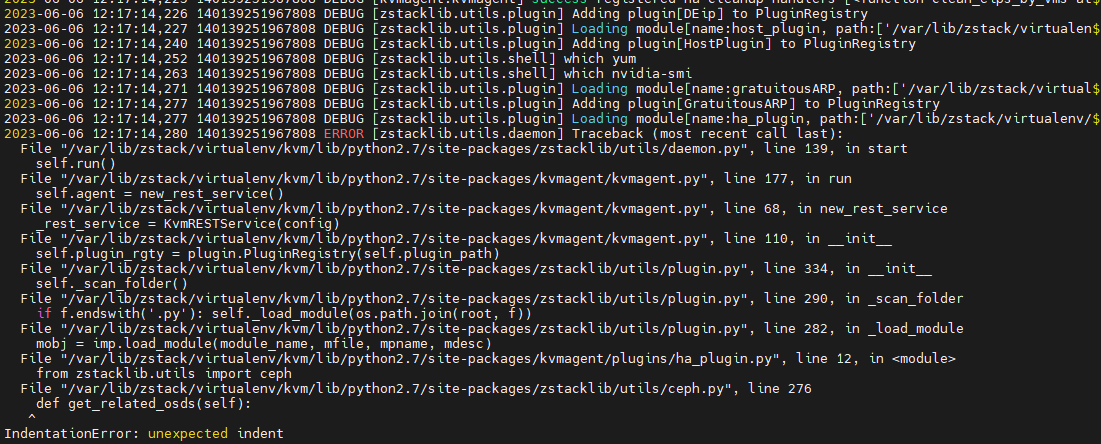
\includegraphics[width=0.8\textwidth]{ZSTAC-56389.png}
                \caption{zstack-kvmagent.log}
            \end{figure}
        \end{onlyenv}
        \item<2-> 有助于查找动态测试过程找不到的缺陷\\
        比如一些很难覆盖到的分支组合
    \end{itemize}
\end{frame}

\begin{frame}{静态分析应用}
    静态分析是一项通用的技术,不是单单为测试而生的。
    有着各种应用:

    \begin{itemize}
        \item 程序可靠性:\\
        {\kaishu 内存泄漏、数组越界访问\ldots}
        \item 程序安全性:\\
        {\kaishu 隐私信息泄露、注入攻击\ldots}
        \item 编译优化:\\
        {\kaishu 常量折叠、代码移动\ldots}
        \item 程序理解:\\
        {\kaishu 类型推导、IDE提示\ldots}
    \end{itemize}
\end{frame}

\section{静态分析基础}

\begin{frame}{静态分析是什么?}
    \begin{definition}[静态分析]
        在\textbf{不执行程序}的情况下对程序进行分析,以了解程序的程序的行为并确定它是否满足某些属性。
    \end{definition}
    \begin{itemize}
        \item 是否有可能出现数组越界访问?
        \item 是否存在死代码?
        \item 是否存在隐私信息泄露?
        \item \ldots
    \end{itemize}
\end{frame}

\begin{frame}{静态分析的局限性}
    \begin{theorem}[莱斯定理]
        \textbf{递归可枚举}语言的任何\textbf{非平凡}的性质,都是\textbf{不可判定}的。
    \end{theorem}
    \note{递归可枚举:图灵完备 - 不完备的DSL}
    \note{非平凡:动态运行时性质 - 语言子集}
    \note{不可判定 - 允许回答不知道/放宽}
    即完美(Sound \& Complete)的静态分析是不存在的。
    \onslide<2->{
        \begin{itemize}
            \item Sound:拒绝漏报\onslide<3>{(通常可以接受)}
            \item \alt<3>{\sout{Complete:拒绝误报}}{Complete:拒绝误报}
        \end{itemize}
        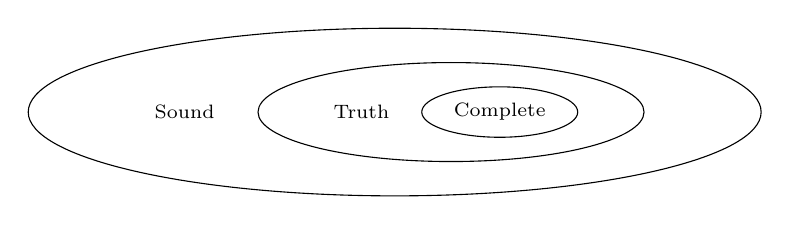
\begin{tikzpicture}[font=\scriptsize]
            \node[draw, ellipse](complete){Complete};
            \node[left=8pt of complete](truthl){Truth};
            \node[draw, ellipse, fit=(complete) (truthl)](truthr) {};
            \node[left=12pt of truthr](soundl){Sound};
            \node[draw, ellipse, fit=(truthr) (soundl)](soundr) {};
        \end{tikzpicture}
    }
\end{frame}

\begin{frame}{静态分析的方法}
    \begin{block}{实用的静态分析原则}
        在确保 soundness 的前提下,在分析的准确度和速度之间做出有效的平衡
    \end{block}
    \begin{itemize}
        \item 抽象:把具体域的值映射到抽象域的值。
        \item 近似:在抽象层面定义转移函数。
    \end{itemize}
    \onslide<2>{根据问题和可用的条件确定。\\
    例:符号执行 > (全局)抽象解释 > (局部)抽象解释}
\end{frame}

\section{数据流分析}

\begin{frame}{编译过程}
    \begin{columns}[c]
        \begin{column}{0.55\textwidth} 
            \begin{tikzpicture}[font=\footnotesize,
                    stage/.style={rectangle, text centered, draw},
                    actor/.style={font=\scriptsize},
                    analy/.style={font=\scriptsize},
                    arrow/.style={draw,thick,-stealth},
                    connect/.style={draw,dashed},
                ]
                \onslide<1->{\node[stage](src) {源代码};}
        
                \onslide<2->{
                \node[stage, below=14pt of src](token) {token流};
                \path[arrow] (src) -- node[actor, right](lexer){Lexer} (token);
                \node[analy, right=60pt of lexer.west](lexical) {词法分析};
                \path[connect] (lexer) -- (lexical);
                }
                
                \onslide<3->{
                \node[stage, below=14pt of token](ast) {语法树};
                \path[arrow] (token) -- node[actor, right](parser){Parser} (ast);
                \node[analy, right=60pt of parser.west](syntax) {句法分析};
                \path[connect] (parser) -- (syntax);
                }
                
                \onslide<4->{
                \node[stage, below=14pt of ast](tast) {(标注了的)语法树};
                \path[arrow] (ast) -- node[actor, right](typer){Type Checker} (tast);
                \node[analy, right=60pt of typer.west](semantic) {语法分析};
                \path[connect] (typer) -- (semantic);
                }
                
                \onslide<5->{
                \node[stage, below=14pt of tast](ir) {中间表示\only<6>{(计算流图)}};
                \path[arrow] (tast) -- node[actor, right](translator){Translator} (ir);
                
                \node[stage, below=14pt of ir](raw) {机器码};
                \path[arrow] (ir) -- node[actor, right](codegen){Code Generator} (raw);
                }

                \onslide<6>{
                \node[analy, right=60pt of ir.center](static) {语义(静态)分析};
                \path[connect] (ir) -- (static);
                }
            \end{tikzpicture}
        \end{column}
        \begin{column}{0.45\textwidth}
            \begin{onlyenv}<1>
            \begin{block}{例:代码片段}
                \footnotesize\ttfamily
do\\
\ \ \ \ i = i + 1\\
while(a[i] < v);
            \end{block}
            \end{onlyenv}
            \begin{onlyenv}<2>
            \begin{block}{Token stream}
                \footnotesize\ttfamily
\fbox{do}\\
\fbox{i} \fbox{=} \fbox{i} \fbox{+} \fbox{1}\\
\fbox{while} \fbox{(} \fbox{a} \fbox{[} \fbox{i} \fbox{]} \fbox{<} \fbox{v} \fbox{)} \fbox{;}
            \end{block}
            \end{onlyenv}
            \begin{onlyenv}<3-4>
            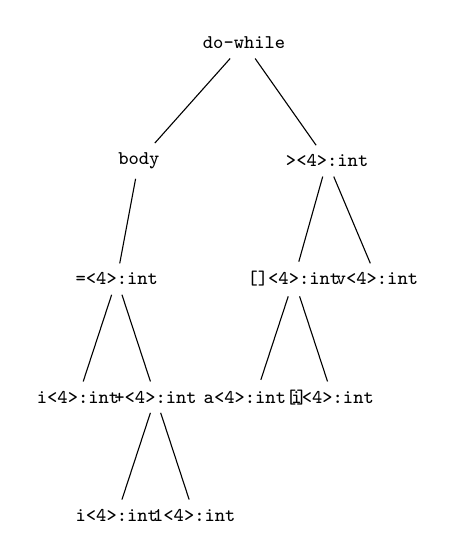
\begin{tikzpicture}[font=\scriptsize\ttfamily,%width=\textwidth
                level 1/.style={sibling distance=60pt},
                level 2/.style={sibling distance=36pt},
                level 3/.style={sibling distance=28pt}
            ]
                \node {do-while}
                  child {node[xshift=-8pt] {body}
                    child {node[xshift=-8pt] {=\only<4>{:int}}
                      child {node {i\only<4>{:int}}}
                      child {node {+\only<4>{:int}}
                        child {node {i\only<4>{:int}}}
                        child {node {1\only<4>{:int}}}
                      }
                    }
                  }
                  child {node {>\only<4>{:int}}
                    child {node[xshift=6pt] {[]\only<4>{:int}}
                      child {node {a\only<4>{:int[]}}}
                      child {node {i\only<4>{:int}}}
                    }
                    child {node {v\only<4>{:int}}}
                  };
            \end{tikzpicture}
            \end{onlyenv}
            \begin{onlyenv}<5>
            \begin{block}{三地址码}
                \footnotesize\ttfamily
1: i = i + 1\\
2: t1 = a[i]\\
3: if t1 < v goto 1
            \end{block}
            \end{onlyenv}
            \begin{onlyenv}<6>
            \begin{tikzpicture}[font=\footnotesize,
                block/.style={rectangle, drop shadow, text ragged left, fill=white, draw},
                line/.style={font=\footnotesize\ttfamily, text ragged left},
                arrow/.style={draw,thick,-stealth},
                arrow0/.style={draw,thick},
            ]
            \node[block](entry){入口};
            \node[line, below=of entry](blk1) {1: i = i + 1};
            \node[line, below=2pt of blk1](blk2) {2: t1 = a[i]};
            \node[line, below=2pt of blk2](blk3) {3: if t1 < v goto 1};
            \begin{scope}[on background layer]
                \node[block,fit=(blk1) (blk2) (blk3)] (body) {};
            \end{scope}
            \node[block, below=of blk3](exit){出口};
            \path[arrow] (entry) -- (body);
            \path[arrow] (body) -- (exit);
            \path[arrow0] (blk3) -| ([xshift=6pt, yshift=6pt] body.north east);
            \path[arrow] ([xshift=6pt, yshift=6pt] body.north east) -| ([xshift=4pt] body);
            \end{tikzpicture}
            \end{onlyenv}
        \end{column}
    \end{columns}
\end{frame}

\begin{frame}{数据流分析基础}
    在数据流分析应用中,将每一个程序点与一个表示该点所有观测到的程序状态集合的抽象数据流值联系起来。

    \begin{columns}[t]
    \begin{column}{0.32\textwidth}
        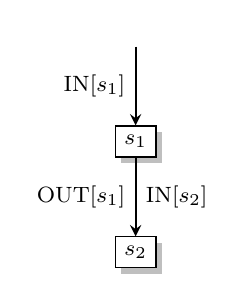
\begin{tikzpicture}[font=\footnotesize,
                block/.style={rectangle, drop shadow, text ragged left, fill=white, draw},
                label/.style={font=\footnotesize},
                arrow/.style={draw,thick,-stealth}
            ]
            \node(entry){};
            \node[block, below=of entry](s1){$s_1$};
            \node[block, below=of s1](s2){$s_2$};
            \path[arrow] (entry) -- node[left](in1){$\IN[s_1]$} (s1);
            \path[arrow] (s1) -- node[left](out1){$\OUT[s_1]$} node[right](in2){$\IN[s_2]$} (s2);
        \end{tikzpicture}
        \par\footnotesize $\IN[s_2]=\OUT[s_1]$
    \end{column}
    \begin{column}{0.32\textwidth}
        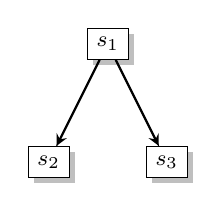
\begin{tikzpicture}[font=\footnotesize,
                block/.style={rectangle, drop shadow, text ragged left, fill=white, draw},
                label/.style={font=\footnotesize},
                arrow/.style={draw,thick,-stealth}
            ]
            \node[block](s1){$s_1$}
            child {node[block](s2){$s_2$}}
            child {node[block](s3){$s_3$}};
            \path[arrow] (s1) -- (s2);
            \path[arrow] (s1) -- (s3);
        \end{tikzpicture}
        \par\footnotesize $\IN[s_2]=\IN[s_3]=\OUT[s_1]$
    \end{column}
    \begin{column}{0.32\textwidth}
        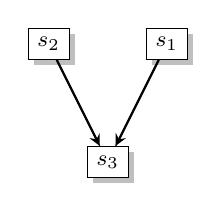
\begin{tikzpicture}[font=\footnotesize,
                block/.style={rectangle, drop shadow, text ragged left, fill=white, draw},
                label/.style={font=\footnotesize},
                arrow/.style={draw,thick,-stealth}
            ]
            \node[block](s3){$s_3$} [grow=up]
            child {node[block](s1){$s_1$}}
            child {node[block](s2){$s_2$}};
            \path[arrow] (s1) -- (s3);
            \path[arrow] (s2) -- (s3);
        \end{tikzpicture}
        \par\footnotesize $\IN[s_3]=\OUT[s_1]\wedge{}\OUT[s_2]$
    \end{column}
    \end{columns}
\end{frame}

\begin{frame}{定义可达性分析}
    \begin{definition}[定义可达性]
        在程序点$p$的一条定义$d$可以\textbf{到达}程序点$q$,如果存在一条由$p$到$q$的路径且定义$d$不会在路径中被覆盖。
    \end{definition}
    \note{应用:消除不必要的变量分配(优化)/检查遗漏(诊断)/哑定义检查未定义变量(诊断)}
    \pause
    \begin{itemize}
        \item 抽象域:每个变量的定义在程序点是否可达\note{bitvector}
        \item 状态转移函数:对于每条形如v=rhs的定义,在这条语句之后,都产生了当前这个定义,并消除了v的所有其他定义
        \item 控制流交点:取并集(只要存在一条路径)
    \end{itemize}
\end{frame}

\begin{frame}{定义可达性分析}
    \begin{block}{定义可达性分析算法}
        \begin{algorithmic}
            \State $\OUT[entry]\gets{}\emptyset{}$
            \ForEach{基本块 $B/entry$}
            \State $\OUT[B]\gets{}\emptyset$
            \EndFor
            \While{任意 $\OUT$ 发生改变}
            \ForEach{基本块 $B/entry$}
            \State $\IN[B]\gets{}\bigcup_{P \pred{} B}\OUT[P]$
            \State $\OUT[B]\gets{}\mathrm{gen}_B\cup(\IN[B]-kill_B)$
            \EndFor
            \EndWhile
        \end{algorithmic}
    \end{block}
\end{frame}

\begin{frame}{定义可达性分析:例子}
    \begin{tikzpicture}[font=\footnotesize,
            block/.style={rectangle, text ragged left, fill=white, draw},
            line/.style={font=\footnotesize\ttfamily, text ragged left},
            value/.style={font=\tiny\ttfamily},
            arrow/.style={draw,thick,-stealth},
            arrow0/.style={draw,thick},
        ]
        \node[block](entry){入口};
        \node[line, below=10pt of entry](d1){D1: \ttfamily x=p-1};
        \node[line, below=2pt of d1](d2){D2: \ttfamily y=q+1};
        \node[line, below=16pt of d2](d3){D3: \ttfamily m=k*2};
        \node[line, below=2pt of d3](d4){D4: \ttfamily y=q-3};
        \node[line, below=16pt of d4, xshift=-30pt](d5){D5: \ttfamily x=5};
        \node[line, below=2pt of d5](d6){D6: \ttfamily z=3};
        \node[line, below=20pt of d4, xshift=30pt](d7){D7: \ttfamily x=m+5};
        \node[line, below=16pt of d6, xshift=30pt](d8){D8: \ttfamily z=2*p};
        \begin{scope}[on background layer]
            \node[block, fit=(d1) (d2)](b1){};
            \node[block, fit=(d3) (d4)](b2){};
            \node[block, fit=(d7)](b3){};
            \node[block, fit=(d5) (d6)](b4){};
            \node[block, fit=(d8)](b5){};
        \end{scope}
        \node[right=2pt of b1]{B1};
        \node[right=2pt of b2]{B2};
        \node[right=2pt of b3]{B3};
        \node[above=2pt of b4, xshift=-12pt]{B4};
        \node[right=2pt of b5]{B5};
        \node[block, below=10pt of b5](exit){出口};
        \path[arrow] (entry) -- node[value, right]{
            \only<2->{0000 0000}
        } (b1);
        \path[arrow] (b1) -- node[value, right]{
            \only<2>{0000 0000}
            \only<3->{\alert<3>{1100 0000}}
        } (b2);
        \path[arrow] (b2) -- node[value, right]{
            \only<2-3>{0000 0000}
            \only<4-8>{\alert<4>{1011 0000}}
            \only<9->{\alert<9>{1011 1100}}
        } (b3);
        \path[arrow] (b2) -- node[value, left]{
            \only<2-3>{0000 0000}
            \only<4-8>{\alert<4>{1011 0000}}
            \only<9->{\alert<9>{1011 1100}}
        } (b4);
        \path[arrow] (b3) -- node[value, right]{
            \only<2-4>{0000 0000}
            \only<5-9>{\alert<5>{0011 0010}}
            \only<10->{\alert<10>{0011 1010}}
        } (b5);
        \path[arrow] (b4) -- node[value, left]{
            \only<2-5>{0000 0000}
            \only<6->{\alert<6,10>{0011 1100}}
        } (b5);
        \path[arrow] (b4.south west) .. controls +(-30pt, -10pt) and +(-10pt, 30pt) .. (b2.north west);
        \path[arrow] (b5) -- node[value, right]{
            \only<2-6>{0000 0000}
            \only<7->{\alert<7>{0011 1101}}
        } (exit);
        \node[value, above=1pt of d8]{
            \only<7>{\alert{$\cup{}$: 0011 1101}}
        };
        \node[value, left=3pt of d3]{
            \only<8,9>{\alert<8>{$\cup{}$: 1111 1100}}
        };
    \end{tikzpicture}
\end{frame}

\begin{frame}{数据流分析}
    \begin{table}[htb]
        \centering
        \caption{数据流分析比较}
        \begin{tabular}{cccc}
            \toprule
            分析应用 & 到达定义 & 存活变量 & 可用表达式\\
            \midrule
            论域 & 定义的集合 & 变量的集合 & 表达式的集合\\
            方向 & 前向 & 反向 & 前向 \\
            边界条件 & $\OUT[entry]=\emptyset$ & $\IN[exit]=\emptyset$ & $\OUT[entry]=\emptyset$ \\
            初始状态 & $\OUT[B]=\emptyset$ & $\IN[B]=\emptyset$ & $\OUT[B]=U$ \\
            传递函数 & \multicolumn{3}{c}{$\OUT[B]=gen_B\cup(\IN[B]-kill_B)$} \\
            合并操作 & $\bigcup$ & $\bigcup$ & $\bigcap$ \\
            \bottomrule
        \end{tabular}
    \end{table}
\end{frame}

\appendix
\section{\appendixname}

\begin{frame}{Q\&A}
    \begin{itemize}
        \item 如何利用定义可达性分析检查可能未初始化的变量?\note{哑定义}
        \item 算法中基本块的选取顺序会对结果有影响吗?
    \end{itemize}
\end{frame}

\begin{frame}
    \Huge\center 谢谢大家
\end{frame}
    

\end{document}
